\documentclass[12pt, a4paper]{article}

% Preamble: Essential packages
\usepackage[margin=2.5cm]{geometry}
\usepackage{amsmath}
\usepackage{amssymb}
\usepackage{graphicx}
\usepackage{tikz}
\usepackage{microtype} % For better typesetting
\usepackage{fontawesome5} % For rocket icon
\usepackage{hyperref}
\hypersetup{
    colorlinks=true,
    linkcolor=blue,
    filecolor=magenta,      
    urlcolor=cyan,
}

% TikZ library for arrows and intersections
\usetikzlibrary{arrows.meta, intersections}

% Title setup
\title{Concise Notes and Solutions for Special Relativity Problems}
\author{Prepared for a 1-Hour Teaching Session}
\date{\today}

\begin{document}
\maketitle
\tableofcontents
\newpage

\section{Teaching Notes: Special Relativity in a Nutshell \faRocket}

This guide covers the essential concepts needed to solve the provided SPhO problems. We'll focus on the core ideas and equations.

\subsection{The Two Postulates}
Special Relativity is built on two simple but revolutionary ideas:
\begin{enumerate}
    \item \textbf{The Principle of Relativity:} The laws of physics are the same in all inertial (non-accelerating) frames of reference.
    \item \textbf{The Constancy of the Speed of Light:} The speed of light in a vacuum, $c$, is the same for all inertial observers, regardless of the motion of the light source or the observer.
\end{enumerate}

\subsection{Key Equations \& Concepts}

\subsubsection{The Lorentz Factor ($\gamma$)}
This factor appears in almost every relativistic calculation. It measures how much time, length, and mass are altered by motion.
$$ \gamma = \frac{1}{\sqrt{1 - \frac{v^2}{c^2}}} $$
Since $v$ is always less than $c$, \textbf{$\gamma$ is always greater than or equal to 1}.

\subsubsection{Time Dilation}
Moving clocks run slow as seen by a stationary observer.
\begin{itemize}
    \item \textbf{Proper Time ($\Delta t_0$):} This is the time interval between two events measured by an observer who sees the events occur at the \textbf{same location}. It's the "shortest" possible time measurement.
    \item \textbf{Dilated Time ($\Delta t$):} This is the time interval measured by an observer moving relative to the events.
\end{itemize}
$$ \Delta t = \gamma \Delta t_0 $$

\subsubsection{Length Contraction}
Objects appear shorter in the direction they are moving, as seen by a stationary observer.
\begin{itemize}
    \item \textbf{Proper Length ($L_0$):} The length of an object measured in its own rest frame. It's the "longest" possible length measurement.
    \item \textbf{Contracted Length ($L$):} The length measured by an observer moving relative to the object.
\end{itemize}
$$ L = \frac{L_0}{\gamma} $$

\subsubsection{Lorentz Transformations}
These equations transform the coordinates of an event from one inertial frame (S) to another (S') moving at a velocity $v$ along the x-axis.
\begin{align*}
    x' &= \gamma (x - vt) \\
    t' &= \gamma \left(t - \frac{vx}{c^2}\right)
\end{align*}
A key consequence is the \textbf{Relativity of Simultaneity}: two events that are simultaneous in one frame ($t_1 = t_2$) are \textbf{not} necessarily simultaneous in another frame ($t'_1 \neq t'_2$) if they occur at different locations ($x_1 \neq x_2$).

\subsubsection{Relativistic Velocity Addition}
Velocities don't simply add up. If object A moves at $u$ and frame B moves at $v$ (both relative to a lab frame), the velocity of A as seen from B ($u'$) is:
$$ u' = \frac{u - v}{1 - \frac{uv}{c^2}} $$

\subsubsection{Relativistic Energy and Momentum}
\begin{itemize}
    \item \textbf{Heisenberg's Uncertainty Principle:} $\Delta x \Delta p \ge \frac{\hbar}{2} \implies p_{\text{min}} \approx \frac{\hbar}{\Delta x}$
    \item \textbf{Energy-Momentum Relation:} $E^2 = (pc)^2 + (m_0c^2)^2$
    \item \textbf{Kinetic Energy ($K$):} $K = E - m_0c^2 = \sqrt{(pc)^2 + (m_0c^2)^2} - m_0c^2$
\end{itemize}

\newpage
\section{Minkowski Spacetime Diagrams}
Spacetime diagrams are essential tools for visualizing relativistic phenomena. Time is plotted on the vertical axis (as $ct$) and one spatial dimension on the horizontal axis (as $x$). The path of an object through spacetime is called its \textbf{worldline}.

\subsection{Visualizing Time Dilation}
Proper time ($\Delta t_0$) is the time between two events (E1, E2) that occur at the \textbf{same location} in a frame (S'). An observer in a stationary frame (S) measures a longer time ($\Delta t$) between these same two events because the events now occur at different locations in their frame.

\begin{figure}[htbp]
\centering
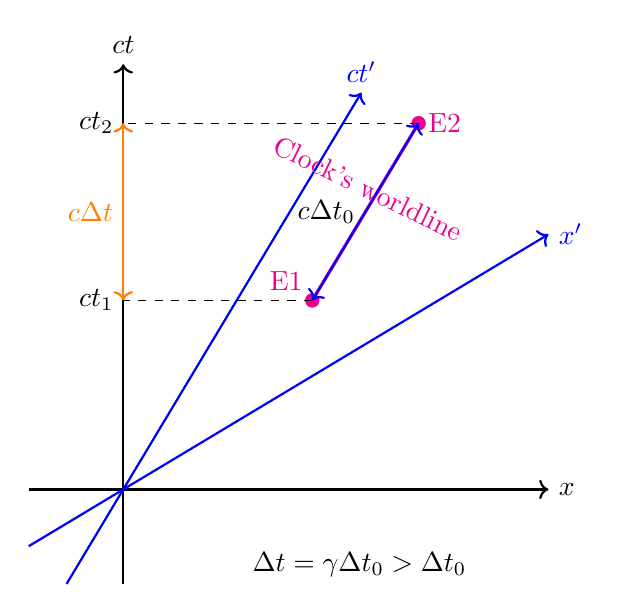
\begin{tikzpicture}[scale=1.2]
    \def\v{0.6} % velocity v/c
    \def\g{1.25} % gamma
    
    % S frame axes (black)
    \draw[->, thick] (-1,0) -- (4.5,0) node[right] {$x$};
    \draw[->, thick] (0,-1) -- (0,4.5) node[above] {$ct$};
    
    % S' frame axes (blue) - EXTENDED
    \draw[->, blue, thick] (-1, -1*\v) -- (4.5, 4.5*\v) node[right] {$x'$};
    \draw[->, blue, thick] (-1*\v, -1) -- (4.2*\v, 4.2) node[above] {$ct'$};

    % Events E1 and E2 for a clock at rest in S' at a constant position x'=1.
    \def\xprime{1.0}
    \def\ctprimeone{1.0}
    \def\ctprimetwo{2.5}
    
    % Transform coordinates from S' to S to plot the points
    \coordinate (E1) at ({\g*(\xprime + \v*\ctprimeone)}, {\g*(\ctprimeone + \v*\xprime)});
    \coordinate (E2) at ({\g*(\xprime + \v*\ctprimetwo)}, {\g*(\ctprimetwo + \v*\xprime)});

    % Draw the clock's worldline (magenta)
    \draw[magenta, very thick] (E1) -- (E2);
    \filldraw[magenta] (E1) circle (2pt) node[above left] {E1};
    \filldraw[magenta] (E2) circle (2pt) node[right] {E2};
    \node[magenta, above, rotate={atan(\v)*180/pi}] at (2.5, 3.0) {Clock's worldline};
    
    % Proper Time in S'
    \draw[<->, blue, thick] (E1) -- (E2) node[midway, left, black] {$c\Delta t_0$};
    
    % Dilated Time in S
    \draw[dashed] (E1) -- (E1 -| 0,0) coordinate (t1);
    \draw[dashed] (E2) -- (E2 -| 0,0) coordinate (t2);
    \node[left] at (t1) {$ct_1$};
    \node[left] at (t2) {$ct_2$};
    
    \draw[<->, thick, orange] (t1) -- (t2) node [midway, left] {$c\Delta t$};
    
    \node at (2.5, -0.8) {$\Delta t = \gamma \Delta t_0 > \Delta t_0$};
\end{tikzpicture}
\caption{Minkowski diagram illustrating \textbf{Time Dilation}. The two events, E1 and E2, occur at the same location in the moving frame S' (blue), so the time between them is proper time, $\Delta t_0$. In the stationary frame S (black), the events are separated by a longer time, the dilated time $\Delta t$.}
\end{figure}

\subsection{Visualizing Length Contraction}
Proper length ($L_0$) is the length of an object measured in its own rest frame (S'). To measure its length in a stationary frame (S), an observer must record the positions of its two ends ($x_A$ and $x_B$) \textbf{simultaneously} (at the same time $t$). This measured length ($L$) is always shorter than the proper length.

\begin{figure}[htbp]
\centering
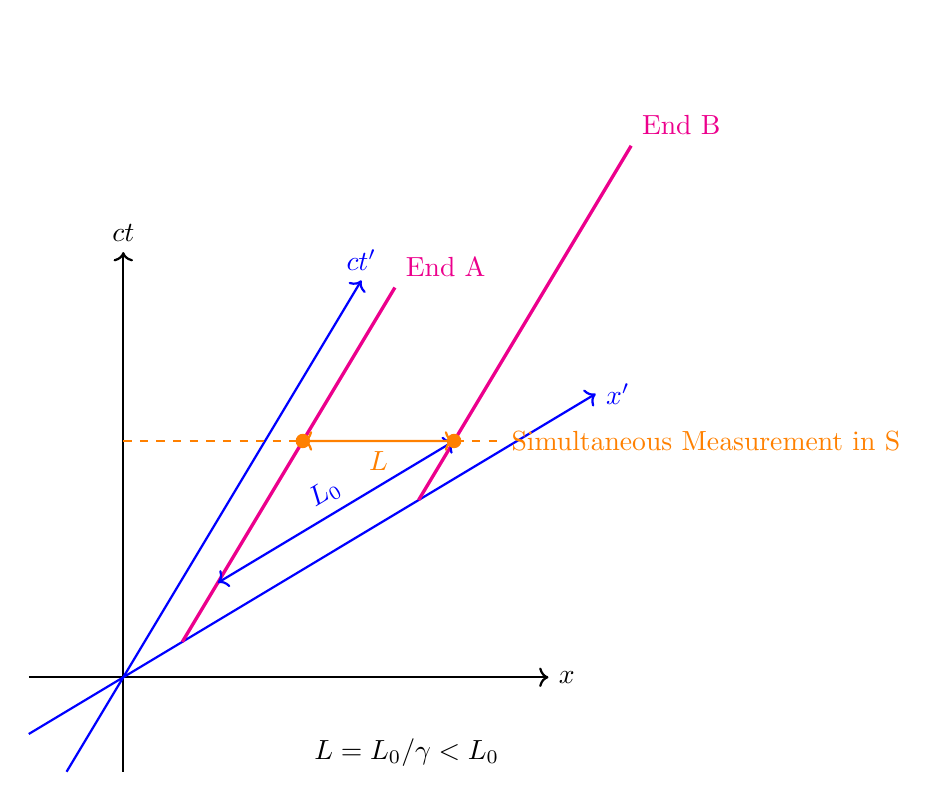
\begin{tikzpicture}[scale=1.2]
    \def\v{0.6} % velocity v/c
    \def\g{1.25} % gamma
    
    % S frame axes (black)
    \draw[->, thick] (-1,0) -- (4.5,0) node[right] {$x$};
    \draw[->, thick] (0,-1) -- (0,4.5) node[above] {$ct$};
    
    % S' frame axes (blue) - EXTENDED
    \draw[->, blue, thick] (-1, -1*\v) -- (5, 5*\v) node[right] {$x'$};
    \draw[->, blue, thick] (-1*\v, -1) -- (4.2*\v, 4.2) node[above] {$ct'$};

    % Worldlines of the ends of a rod at rest in S'
    \def\xprimeA{0.5}
    \def\xprimeB{2.5}

    % Define the worldlines as paths for finding intersections
    \path[name path=worldlineA] ({\g*(\xprimeA + \v*(-1))}, {\g*(-1 + \v*\xprimeA)}) -- ({\g*(\xprimeA + \v*4)}, {\g*(4 + \v*\xprimeA)});
    \path[name path=worldlineB] ({\g*(\xprimeB + \v*(-1))}, {\g*(-1 + \v*\xprimeB)}) -- ({\g*(\xprimeB + \v*4)}, {\g*(4 + \v*\xprimeB)});

    % Draw the visible parts of the worldlines
    \draw[magenta, very thick] ({\g*(\xprimeA + \v*0)}, {\g*(0 + \v*\xprimeA)}) -- ({\g*(\xprimeA + \v*3)}, {\g*(3 + \v*\xprimeA)}) node[above right] {End A};
    \draw[magenta, very thick] ({\g*(\xprimeB + \v*0)}, {\g*(0 + \v*\xprimeB)}) -- ({\g*(\xprimeB + \v*3)}, {\g*(3 + \v*\xprimeB)}) node[above right] {End B};

    % Proper Length in S'
    \coordinate (P1) at ({\g*(\xprimeA + \v*0.5)}, {\g*(0.5 + \v*\xprimeA)});
    \coordinate (P2) at ({\g*(\xprimeB + \v*0.5)}, {\g*(0.5 + \v*\xprimeB)});
    \draw[<->, blue, thick] (P1) -- (P2) node[midway, above, sloped] {$L_0$};
    
    % Contracted Length in S
    \path[name path=simul_line] (-1, 2.5) -- (4.5, 2.5);
    \draw[dashed, orange, thick] (0, 2.5) -- (4, 2.5) node[right] {Simultaneous Measurement in S};
    
    % Find intersections
    \path[name intersections={of=worldlineA and simul_line, by=MA}];
    \path[name intersections={of=worldlineB and simul_line, by=MB}];
    \filldraw[orange] (MA) circle (2pt);
    \filldraw[orange] (MB) circle (2pt);
    
    \draw[<->, thick, orange] (MA) -- (MB) node[midway, below] {$L$};
    
    \node at (3, -0.8) {$L = L_0 / \gamma < L_0$};
\end{tikzpicture}
\caption{Minkowski diagram illustrating \textbf{Length Contraction}. A rod of proper length $L_0$ is at rest in the moving frame S' (its ends follow the magenta worldlines). To measure its length in frame S, the positions of the ends are noted at the same time. The resulting distance $L$ is shorter than $L_0$.}
\end{figure}

\newpage

\section{Problem Solutions}

\subsection{SR1: SPhO 2024 (Spacecraft Journey)}
\textbf{Question:} \textit{A spacecraft is moving at a constant velocity v relative to an observer on Earth. The spacecraft is traveling in a straight line from point A to point B, which are 10 light-years apart as measured in Earth's frame.}
\vspace{1em}

\textbf{(a)} \textit{Calculate the time it takes for the spacecraft to travel from point A to point B as measured by the observer on Earth if the velocity of the spacecraft is 0.8c, where c is the speed of light.}
\vspace{1em}
This is a straightforward calculation.
Distance $d = 10 \text{ light-years} = 10c \cdot \text{years}$. Velocity $v = 0.8c$.
$$ t = \frac{d}{v} = \frac{10c \cdot \text{years}}{0.8c} = \mathbf{12.5 \textbf{ years}} $$

\textbf{(b)} \textit{Determine the time experienced by a clock on the spacecraft for the journey from A to B.}
\vspace{1em}
The clock on the spacecraft measures the proper time $\Delta t_0$. The time measured on Earth is the dilated time $\Delta t$. First, find $\gamma$:
$$ \gamma = \frac{1}{\sqrt{1 - (0.8)^2}} = \frac{1}{\sqrt{1 - 0.64}} = \frac{1}{\sqrt{0.36}} = \frac{1}{0.6} = \frac{5}{3} $$
$$ \Delta t_0 = \frac{\Delta t}{\gamma} = \frac{12.5}{5/3} = 12.5 \times \frac{3}{5} = \mathbf{7.5 \textbf{ years}} $$

\textbf{(c)} \textit{Suppose a light signal is sent from point A to point B just as the spacecraft passes point A. How much time does it take for the signal to reach point B as measured by: i. The observer on Earth. ii. The astronaut on the spacecraft.}
\vspace{1em}
i. \textbf{On Earth:} Light travels at $c$, so the time is $t = \frac{d}{c} = \frac{10c \cdot \text{years}}{c} = \mathbf{10 \textbf{ years}}$.
ii. \textbf{On the spacecraft:} According to the second postulate, the astronaut also measures the light's speed as $c$. However, the distance from A to B is contracted in the spacecraft's frame:
$$ d_0 = \frac{d}{\gamma} = \frac{10 \text{ ly}}{5/3} = 6 \text{ light-years} $$
Time measured by astronaut $t_0 = \frac{d_0}{c} = \frac{6c \cdot \text{years}}{c} = \mathbf{6 \textbf{ years}}$.

\textbf{(d)} \textit{Assume that when the spacecraft reaches point B, a signal is sent back to point A. According to the observer on Earth, do the events "spacecraft reaches point B" and "signal reaches point A" occur simultaneously? Explain your reasoning.}
\vspace{1em}
\textbf{No}, the events are not simultaneous. The spacecraft reaches point B at $t = 12.5$ years. A signal sent from B takes 10 years to travel back to A, arriving at $t = 12.5 + 10 = 22.5$ years. These times are clearly different. This illustrates that events separated in space are not generally simultaneous.

\begin{figure}[htbp]
\centering
\begin{tikzpicture}[scale=0.5]
    \draw[->] (-1,0) -- (12,0) node[right] {$x$ (light-years)};
    \draw[->] (0,-1) -- (0,24) node[above] {$ct$ (years)};
    % Spacecraft worldline
    \draw[blue, thick] (0,0) -- (10, 12.5) node[right, black] {Spacecraft};
    \filldraw[blue] (0,0) circle (3pt) node[below left, black] {A (0,0)};
    \filldraw[blue] (10,12.5) circle (3pt) node[above right, black] {B (10, 12.5)};
    % Light signal
    \draw[red, dashed, thick] (0,0) -- (10,10) node[right, black] {Signal A to B};
    % Return signal
    \draw[red, dashed, thick] (10,12.5) -- (0, 22.5) node[above left, black] {Return Signal};
    \filldraw[red] (0,22.5) circle (3pt) node[below left, black, xshift=-2mm] {Signal Arrives at A};
\end{tikzpicture}
\caption{Spacetime diagram for SR1. The blue line is the spacecraft's worldline from A to B. The red dashed lines are the light signals. The arrival at B (12.5 years) and the return signal's arrival at A (22.5 years) are clearly not simultaneous.}
\end{figure}

\newpage

\subsection{SR2: SPhO 2023 (Red and Blue Flash)}
\textbf{Question:} \textit{An observer A in the inertial frame S sees a red flash of light at the origin at time $t=0$ and a blue flash of light at $x=x_{B}$ km and time $t=9.50\mu s$. Another observer B is situated at the origin of another inertial frame $S^{\prime}$ which moves in the direction of increasing x with a speed of v relative to S. The axes of the two inertial frames are parallel at all times and their origins coincide at $t=t^{\prime}=0$. If $v=0.6c$ what is the range of the values of $x_{B}$ so that observer B sees the blue flash before seeing the red flash?}
\vspace{1em}

This problem is a direct application of the Lorentz transformation for time to check the relativity of simultaneity.
We are given two events in frame S:
\begin{itemize}
    \item Red flash: $(x_R, t_R) = (0, 0)$.
    \item Blue flash: $(x_B, t_B) = (x_B, 9.50 \mu s)$.
\end{itemize}
Observer B is in frame S', moving at $v = 0.6c$. In frame S', the time of the red flash is $t'_R = \gamma(t_R - \frac{vx_R}{c^2}) = 0$. The time of the blue flash is $t'_B = \gamma(t_B - \frac{vx_B}{c^2})$.
For B to see the blue flash first, we need $t'_B < t'_R$.
$$ \gamma\left(t_B - \frac{vx_B}{c^2}\right) < 0 \implies t_B < \frac{vx_B}{c^2} $$
Rearranging for $x_B$: $x_B > \frac{c^2 t_B}{v}$.
$$ x_B > \frac{(3 \times 10^8 \text{ m/s})^2 (9.50 \times 10^{-6} \text{ s})}{0.6 \times (3 \times 10^8 \text{ m/s})} = 4750 \text{ m} $$
The range of values is $\mathbf{x_B > 4.75 \textbf{ km}}$.

\begin{figure}[htbp]
\centering
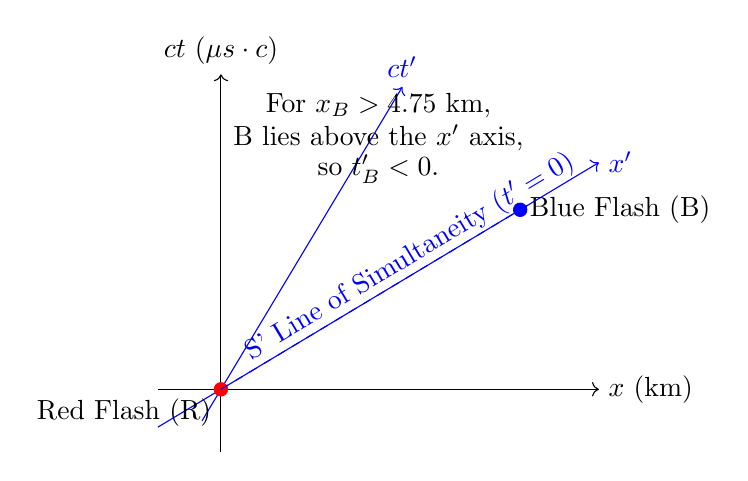
\begin{tikzpicture}[scale=0.8]
    \draw[->] (-1,0) -- (6,0) node[right] {$x$ (km)};
    \draw[->] (0,-1) -- (0,5) node[above] {$ct$ ($\mu s \cdot c$)};
    \def\v{0.6} \def\angle{atan(\v)}
    % S' axes
    \draw[->, blue] (-1,-1*\v) -- (6, 6*\v) node[right] {$x'$};
    \draw[->, blue] (-0.5*\v,-0.5) -- (4.8*\v, 4.8) node[above] {$ct'$};
    % Events
    \filldraw[red] (0,0) circle (3pt) node[below left, black] {Red Flash (R)};
    \filldraw[blue] (4.75, 2.85) circle (3pt) node[right, black] {Blue Flash (B)}; % 9.5us * c = 2.85km
    \node at (2.5, 4.5) {For $x_B > 4.75$ km,};
    \node at (2.5, 4) {B lies above the $x'$ axis,};
    \node at (2.5, 3.5) {so $t'_B < 0$.};
    % Line of simultaneity for S'
    \draw[blue, dashed] (0,0) -- (5, 5*\v);
    \node[blue, rotate=\angle] at (3, 3*\v+0.3) {S' Line of Simultaneity ($t'=0$)};
\end{tikzpicture}
\caption{Spacetime diagram for SR2. The red flash is at the origin. The blue flash (B) must occur in the region above the tilted blue $x'$ axis for its time coordinate $t'_B$ to be negative (i.e., occur before the red flash in frame S').}
\end{figure}

\newpage

\subsection{SR3: SPhO 2022 (Density and Spaceships)}
\textbf{(a)} \textit{A cube lies with one of its faces on the x-y plane and three of its edges along the x, y \& z axes. The cube starts to slide horizontally along the x-axis with constant speed v. It is found that as a result of the motion, the density of the material of the cube appears to increase by 25\%. Calculate the value of v.}
\vspace{1em}
Density $\rho = \frac{m}{V}$. The mass $m$ is invariant. The volume contracts due to motion along one axis.
Proper volume $V_0 = l^3$. Contracted volume $V = \frac{V_0}{\gamma}$. The new density is $\rho' = \frac{m}{V} = \gamma \rho_0$.
Given $\rho' = 1.25 \rho_0$, so $\gamma = 1.25$.
$$ \gamma = \frac{1}{\sqrt{1 - v^2/c^2}} \implies 1.25 = \frac{1}{\sqrt{1 - v^2/c^2}} $$
$$ 1 - \frac{v^2}{c^2} = \frac{1}{1.25^2} = 0.64 \implies \frac{v^2}{c^2} = 0.36 \implies v = \mathbf{0.6c} $$
\vspace{1em}
\textbf{(b)} \textit{An observer in the Earth frame observes two spaceships A and B pass each other in opposite directions. In the inertial frame in which both spaceships are at rest, the lengths of spaceship A and spaceship B are 200 m and 150 m respectively. The observer in the Earth frame measures that the speed of spaceship A is 0.8c and that of spaceship B is 0.6c. As measured by this observer, what is the time interval between the instant when the nose of spaceship A passes the nose of spaceship B and the instant when the tail of spaceship A passes the tail of spaceship B? What is the corresponding time interval measured by an observer sitting at the nose of spaceship A?}
\vspace{1em}
\textbf{In the Earth frame:}
Proper lengths: $L_{0A} = 200$ m, $L_{0B} = 150$ m. Velocities: $v_A = 0.8c$, $v_B = -0.6c$.
Lorentz factors: $\gamma_A = \frac{1}{\sqrt{1-0.8^2}} = \frac{5}{3}$, $\gamma_B = \frac{1}{\sqrt{1-0.6^2}} = \frac{5}{4}$.
Contracted lengths: $L_A = \frac{L_{0A}}{\gamma_A} = 120$ m. $L_B = \frac{L_{0B}}{\gamma_B} = 120$ m.
Event 1: Noses pass at $(x,t)=(0,0)$.
Event 2: Tails pass. $x_{TA}(t) = v_A t - L_A$, $x_{TB}(t) = v_B t + L_B$.
They pass when $x_{TA}(t) = x_{TB}(t)$.
$$ t = \frac{L_A + L_B}{v_A - v_B} = \frac{120 \text{ m} + 120 \text{ m}}{0.8c - (-0.6c)} = \frac{240 \text{ m}}{1.4c} = \mathbf{5.71 \times 10^{-7} \textbf{ s}} $$

\textbf{In spaceship A's frame:}
Use the Lorentz transformation for time, $t' = \gamma_A (t - \frac{v_A x}{c^2})$.
Event 1: $(x_1, t_1) = (0,0) \implies t'_1 = 0$.
Event 2: $(x_2, t_2) = (v_A t - L_A, t)$.
$$ t'_2 = \gamma_A (t_2 - \frac{v_A x_2}{c^2}) = \frac{5}{3} \left(t - \frac{0.8c(0.8ct - 120)}{c^2}\right) $$
$$ t'_2 = \frac{5}{3} \left(t - 0.64t + \frac{96}{c}\right) = \frac{5}{3} \left(0.36t + \frac{96}{c}\right) $$
Substitute $t = 5.714 \times 10^{-7}$ s.
$$ t'_2 = \frac{5}{3} \left(0.36(5.714 \times 10^{-7}) + \frac{96}{3 \times 10^8}\right) = \mathbf{1.71 \times 10^{-7} \textbf{ s}} $$

\begin{figure}[htbp]
\centering
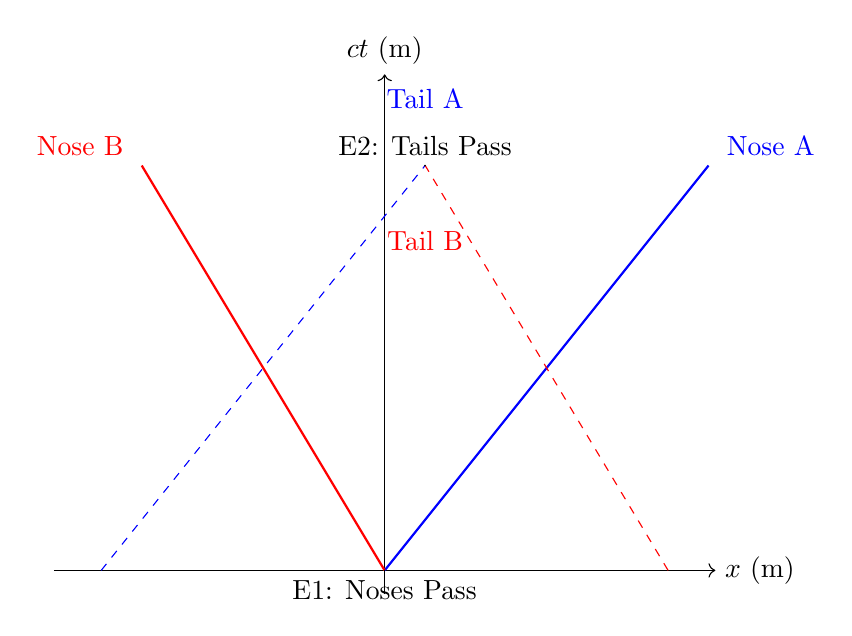
\begin{tikzpicture}[scale=0.03]
    \draw[->] (-140,0) -- (140,0) node[right] {$x$ (m)};
    \draw[->] (0,-10) -- (0,210) node[above] {$ct$ (m)};
    % Worldlines
    \coordinate (ct_end) at (0, 171.4);
    \draw[blue, thick] (0,0) -- (0.8*171.4, 171.4) node[anchor=south west, xshift=1mm] {Nose A};
    \draw[blue, dashed] (-120,0) -- (0.8*171.4-120, 171.4);
    \draw[red, thick] (0,0) -- (-0.6*171.4, 171.4) node[anchor=south east, xshift=-1mm] {Nose B};
    \draw[red, dashed] (120,0) -- (-0.6*171.4+120, 171.4);
    % Events
    \filldraw (0,0) circle (1.5pt) node[below] {E1: Noses Pass};
    \coordinate (E2) at (0.8*171.4-120, 171.4);
    \filldraw (E2) circle (1.5pt);
    % Labels for tails
    \node[above] at (E2) {E2: Tails Pass};
    \node[blue, anchor=south, yshift=6mm] at (E2) {Tail A};
    \node[red, anchor=south, yshift=-12mm] at (E2) {Tail B};
\end{tikzpicture}
\caption{Worldlines of the noses (solid) and tails (dashed) of spaceships A (blue) and B (red) in the Earth frame. Event E1 is the noses passing at the origin. Event E2 is the tails passing.}
\end{figure}

\newpage

\subsection{SR4: SPhO 2021 (Electron in a Nucleus)}
\textbf{Question:} \textit{Calculate the minimum kinetic energy an electron must have in order to be constrained within the nucleus, with a typical nuclear radius of $r=6 \times 10^{-15}$ m. Assume that the uncertainty of this electron's position is equal to the nuclear radius r. Treat the electron relativistically.}
\vspace{1em}

\textbf{Step 1: Find the electron's minimum momentum.}
Use the Heisenberg Uncertainty Principle. $\Delta x = r = 6 \times 10^{-15}$ m.
$$ p \approx \frac{\hbar}{\Delta x} = \frac{1.055 \times 10^{-34} \text{ J}\cdot\text{s}}{6 \times 10^{-15} \text{ m}} = 1.758 \times 10^{-20} \text{ kg}\cdot\text{m/s} $$

\textbf{Step 2: Use the relativistic energy-momentum relation.}
$K = \sqrt{(pc)^2 + (m_e c^2)^2} - m_e c^2$.
Convert terms to MeV: $m_e c^2 = 0.511 \text{ MeV}$.
$$ pc = (1.758 \times 10^{-20})(3 \times 10^8) = 5.274 \times 10^{-12} \text{ J} $$
$$ pc = \frac{5.274 \times 10^{-12} \text{ J}}{1.602 \times 10^{-13} \text{ J/MeV}} = 32.9 \text{ MeV} $$

\textbf{Step 3: Calculate the kinetic energy.}
Notice that $pc \gg m_e c^2$ (32.9 MeV vs 0.511 MeV), so the electron is highly relativistic.
$$ K = \sqrt{(32.9 \text{ MeV})^2 + (0.511 \text{ MeV})^2} - 0.511 \text{ MeV} \approx \mathbf{32.4 \textbf{ MeV}} $$

\subsection{SR5: SPhO 2020 (Muon Decay)}
\textbf{Question:} \textit{Muons are particles which are created in the upper atmosphere via cosmic interactions. These particles travel vertically downward to the surface of the Earth at a speed of 0.995c where c represents the speed of light in vacuum. When muons are at rest, they have a half-life of 1.56$\mu$s. A muon counter is placed at the top of a mountain 2000 m high. The counter records 568 muons in 1 hour.}
\vspace{1em}
\textbf{(i)} \textit{According to classical concepts, what will be the number of muons counted in 1 hour if the counter is placed at the foot of the mountain?}
\vspace{1em}
Time of flight: $t = \frac{d}{v} = \frac{2000 \text{ m}}{0.995 \times 3 \times 10^8 \text{ m/s}} = 6.70 \mu\text{s}$.
Number of half-lives: $n = \frac{t}{T_{1/2}} = \frac{6.70 \mu\text{s}}{1.56 \mu\text{s}} = 4.29$.
Surviving fraction: $N/N_0 = (1/2)^n = (1/2)^{4.29} \approx 0.051$.
Expected count rate: $R = 568 \times 0.051 \approx \mathbf{29 \textbf{ muons/hour}}$.
\vspace{1em}
\textbf{(ii)} \textit{In a typical experiment, a counter placed at the foot of the mountain record 422 muons in 1 hour. Why does the result of this experiment differ so much from your result in part (i)?}
\vspace{1em}
The classical calculation ignores \textbf{time dilation}. The muon's internal clock runs slower from our perspective. Its half-life in our frame is dilated, so fewer muons decay, and more reach the ground.
\vspace{1em}
\textbf{(iii)} \textit{What is the "height" of the mountain according to muons?}
\vspace{1em}
The muons see the mountain's height as length-contracted.
$$ \gamma = \frac{1}{\sqrt{1 - 0.995^2}} \approx 10 $$
Contracted height $H' = \frac{H_0}{\gamma} = \frac{2000 \text{ m}}{10} = \mathbf{200 \textbf{ m}}$.
\vspace{1em}
\textbf{(iv)} \textit{While the muons are travelling downward to the earth, another particle also travels in the same direction with speed 0.9995c. What is the velocity of this particle in the muon's inertial frame?}
\vspace{1em}
Use the velocity addition formula. Earth frame = S, Muon frame = S'.
$v = 0.995c$, $u = 0.9995c$.
$$ u' = \frac{u - v}{1 - \frac{uv}{c^2}} = \frac{0.9995c - 0.995c}{1 - (0.9995)(0.995)} = \frac{0.0045c}{0.0054975} \approx \mathbf{0.819c} $$

\begin{figure}[htbp]
\centering
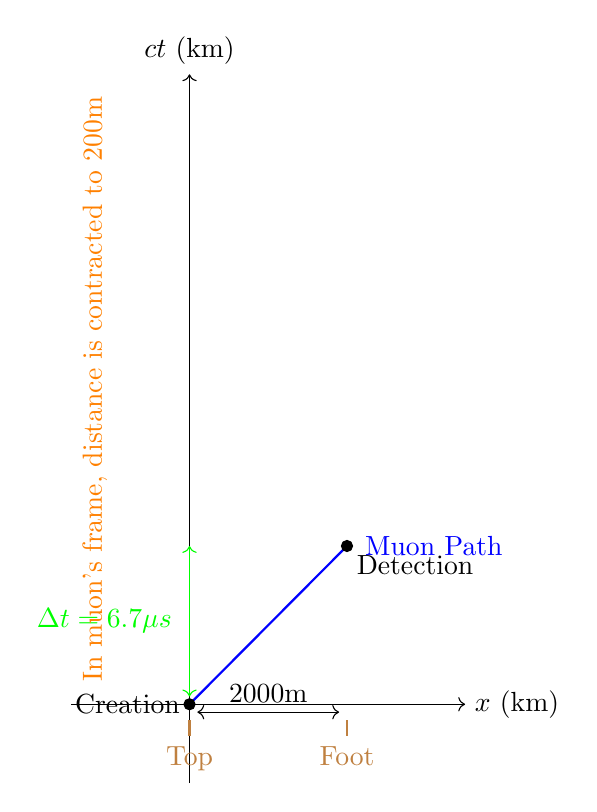
\begin{tikzpicture}[scale=1.0]
    \draw[->] (-1.5,0) -- (3.5,0) node[right] {$x$ (km)};
    \draw[->] (0,-1) -- (0,8) node[above] {$ct$ (km)};
    % Mountain
    \draw[thick, brown] (0,-0.2) -- (0, -0.4) node[below] {Top};
    \draw[thick, brown] (2,-0.2) -- (2,-0.4) node[below] {Foot};
    \draw[<->] (0.1,-0.1) -- (1.9,-0.1) node[midway, above] {2000m};
    % Muon Worldline
    \def\v{0.995}
    \def\t{2.01} % time in km/c
    \draw[blue, thick] (0,0) -- (2, \t) node[right, xshift=1mm] {Muon Path};
    \filldraw (0,0) circle (2pt) node[left] {Creation};
    \filldraw (2, \t) circle (2pt) node[below right] {Detection};
    % Time Dilation
    \draw[<->, green] (0,0.1) -- (0, \t) node[midway, left, anchor=east, xshift=-1mm] {$\Delta t = 6.7 \mu s$};
    % Length Contraction
    \node[orange, rotate=90] at (-1.2, 4) {In muon's frame, distance is contracted to 200m};
\end{tikzpicture}
\caption{Diagram for SR5 showing the muon's worldline from creation to detection. The vertical distance on the $ct$ axis is the dilated time measured on Earth. For the muon, the horizontal distance is contracted.}
\end{figure}

\newpage

\subsection{SR6: SPhO 2019 (Events and Cube Volume)}
\textbf{(a)} \textit{One event occurs at the origin of an inertial frame S at the time $t=0$. Another event occurs at $x=4c, y=z=0, t=5$ sec relative to S.}
\vspace{1em}
\textbf{(i)} \textit{Determine the velocity, relative to S, of the inertial frame S' in which the two events are recorded at the same point in space.}
\vspace{1em}
We need a frame S' where the events occur at the same point ($\Delta x' = 0$).
$$ \Delta x' = \gamma(\Delta x - v \Delta t) = 0 \implies v = \frac{\Delta x}{\Delta t} = \frac{4c}{5\text{ s}} = \mathbf{0.8c} $$
\vspace{1em}
\textbf{(ii)} \textit{What is the time interval between the events in S' frame?}
\vspace{1em}
This is the proper time interval $\Delta t_0$. $\gamma = \frac{1}{\sqrt{1 - (0.8)^2}} = \frac{5}{3}$.
$$ \Delta t' = \Delta t_0 = \frac{\Delta t}{\gamma} = \frac{5 \text{ s}}{5/3} = \mathbf{3 \textbf{ s}} $$
\vspace{1em}
\textbf{(b)} \textit{A cube with sides of length l is moving with one of its sides parallel to the x-axis of an inertial frame S with velocity u. An observer is moving along the x-axis of the inertial frame S with velocity v. Both u \& v are comparable to c, the speed of light. Derive an expression for the volume of the cube as measured by the observer in terms of l, u, v \& c.}
\vspace{1em}
The observer's velocity is $v$, cube's velocity is $u$. Relative velocity is $u' = \frac{u - v}{1 - uv/c^2}$.
The volume is contracted only in the direction of relative motion.
$$ V' = l^2 \cdot \left(l \sqrt{1 - (u')^2/c^2}\right) = l^3 \sqrt{1 - \frac{1}{c^2}\left(\frac{u-v}{1 - uv/c^2}\right)^2} $$
Simplifying the term under the square root:
$$ 1 - \frac{(u')^2}{c^2} = \frac{(1 - uv/c^2)^2 - (u-v)^2/c^2}{(1 - uv/c^2)^2} = \frac{(1-u^2/c^2)(1-v^2/c^2)}{(1-uv/c^2)^2} $$
Therefore, the measured volume is:
$$ V' = \mathbf{l^3 \frac{\sqrt{(1-u^2/c^2)(1-v^2/c^2)}}{|1 - uv/c^2|}} $$

\subsection{SR7: SPhO 2018 (Rocket and Radar)}
\textbf{Question:} \textit{A rocket of proper length 600 m is moving directly away from the earth with uniform velocity. A radar pulse is sent out from the earth and is reflected from the reflectors at the back end and the front end of the rocket. The first reflected radar pulse is received back at the base 5.00 minutes after emission and the second reflected pulse is received 12.0 $\mu$s later.}
\vspace{1em}
\textbf{(a)} \textit{Calculate the distance of the rocket from the earth at the instant the outgoing radar pulse hits the back end reflector.}
\vspace{1em}
Pulse sent at $t=0$, hits back at $t_1$, returns at $T_1 = 300$ s.
The time to travel out and back is equal: $ct_1 = c(T_1 - t_1) \implies t_1 = T_1/2 = 150$ s.
Distance $d = ct_1 = (3 \times 10^8 \text{ m/s})(150 \text{ s}) = \mathbf{4.50 \times 10^{10} \textbf{ m}}$.
\vspace{1em}
\textbf{(b)} \textit{Calculate the velocity of the rocket relative to the earth.}
\vspace{1em}
Time between reflections in Earth frame: $\Delta t_{\text{earth}} = (12.0 \mu\text{s})/2 = 6.0 \mu\text{s}$.
In this time, the distance covered by the light pulse ($c \Delta t_{\text{earth}}$) is equal to the rocket's contracted length ($L_0/\gamma$) plus the distance the rocket travels in that same time ($v \Delta t_{\text{earth}}$).
$$ c \Delta t_{\text{earth}} = \frac{L_0}{\gamma} + v \Delta t_{\text{earth}} $$
Rearranging and solving for $v$ leads to:
$$ \frac{v}{c} = \frac{(\Delta t_{\text{earth}})^2 - (L_0/c)^2}{(\Delta t_{\text{earth}})^2 + (L_0/c)^2} $$
Given $L_0 = 600$ m, so $L_0/c = 2.0 \mu$s.
$$ \frac{v}{c} = \frac{(6.0)^2 - (2.0)^2}{(6.0)^2 + (2.0)^2} = \frac{32}{40} = 0.8 \implies v = \mathbf{0.8c} $$
\vspace{1em}
\textbf{(c)} \textit{Calculate the time interval between the reflections at the back end and front end of the rocket measured in the inertial frame of the rocket.}
\vspace{1em}
In the rocket's frame, the pulse travels the proper length $L_0$ at speed $c$.
$$ \Delta t_{\text{rocket}} = \frac{L_0}{c} = \frac{600 \text{ m}}{3 \times 10^8 \text{ m/s}} = \mathbf{2.0 \mu\textbf{s}} $$
\vspace{1em}
\textbf{(d)} \textit{Explain why the time interval between the reflections in the two frames (i.e. the earth frame and the rocket frame) are not related by the time dilation formula.}
\vspace{1em}
The time dilation formula, $\Delta t = \gamma \Delta t_0$, only applies when $\Delta t_0$ is a \textbf{proper time interval}, meaning the two events occur at the \textbf{same spatial location} in that frame. Here, the two events are "reflection at the back" and "reflection at the front." Since these occur at different locations in both the Earth frame and the rocket frame, neither measured time interval is a proper time, and the simple time dilation formula cannot be used.

\end{document}